\section{Vision-and-Language Navigation}
The idea in~\cite{DBLP:journals/corr/abs-1711-07280} that they might be able to provide general, verbal directions to a robot and have a minimum of an affordable likelihood that it'll do the specified task is one in all the long-held goals of artificial intelligence, and robots.
Despite vital progress, there area unit variety of major technical challenges that require to be over precede robots are going to be able to perform general tasks within the universe. One in all the first needs are going to be new techniques for linking language to vision and action in \emph{unstructured}, \emph{previously unseen environments}. They refer it as Vision-and-Language Navigation (VLN) because of the navigation version of this challenge~\cite{DBLP:journals/corr/abs-1711-07280}.

\begin{figure}[htbp]
    \centering
    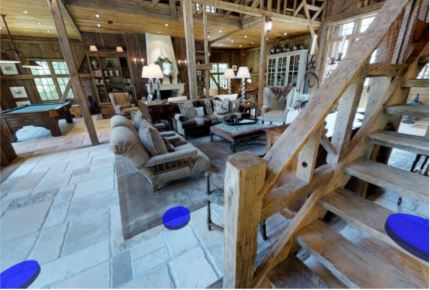
\includegraphics[width=.8\textwidth]{vln}
    \caption{Room-to-Room (R2R) navigation task~\cite{DBLP:journals/corr/abs-1711-07280}}
\end{figure}
\newpage
\subsection*{Instruction}
Head upstairs and walk past the piano through an entryway directly before. Turn right once corridor ends at footage and table. Wait by the moose antlers hanging on the wall.\\

Previous approaches to natural language command of robots have often neglected the visual information processing aspect of the problem. The R2R dataset is the first dataset to evaluate the capability to follow natural language navigation instructions in previously unseen real images at building scale. To explore this task they investigated several baselines and a sequence-to-sequence neural network agent.  The process used to generate R2R is applicable to a host of related vision and language problems, particularly in robotics. 
